

\chapter{Results}

%TODO: I NEED TO TALK ABOUT HYPERPARAMETERS

This chapter reports on the results I have found within this thesis. I will
first report on my investigation of utilitarian online learning models, since
this is relevant to determining which model to use for our regression market.
Then, I will report on results of the market with varying feature spaces,
showing the outcome of the market in toy cases.

Note that whenever I test a model, I also add in a constant feature $1$ on top
of the other features, which acts like the intercept in an ordinary linear
regression.

\section{Utilitarian Online Learning}
\subsection{OCDS}
First, I test the OCDS method against the baseline OLM method in a setup similar
to what is found in the OCDS paper TODO:REF. In this test, I test both OCDS and
OLM as classification methods, and I test their mean accuracy.

The test takes in a dataset of features and associated targets $X,y$. The time
order of these features and targets is shuffled, so that there is no effect of
the order of the features. Then, for every time step, half of the features are
removed, so that methods must handle missing features.

The model first predicts a label for a single time step, and
then trains on that time step. The test pseudocode is displayed in algorithm
\ref{alg:test}. The entire test is run several times, and the mean and standard
deviation of mean accuracy over the dataset is used to create accuracy
confidence intervals.

\begin{algorithm}
  \caption{Pseudocode for testing UOL methods}\label{alg:test}
  \begin{algorithmic}
    \State Permute $X,y$
    \State Initialize model $m$
    \For{$t \in \{0,1,\dots,T\}$}
    \State Create prediction $\hat y_t = m.predict(\mathbf {x}_t)$
    \State Train model $m.train(\mathbf{x}_t,y_t)$
    \EndFor
    \State evaluate model based on predictions $\hat y$
  \end{algorithmic}
\end{algorithm}

I tested OCDS using this approach, along with OLM. I also used a logistic
regression on the same dataset. Logistic regression is the batch learning
variant of a linear classifier using binary cross-entropy loss. I wanted to
investigate a feasible upper bound for predictive accuracy, so I let this
logistic regression train on the entire dataset, and then predict on the entire
dataset as well. Its predictions are then in-sample, meaning that we expect it
to maximize accuracy within the sample. So no other method should be able to
surpass the logistic regression results.

OLM has a hyperparameter in form of a single step size. I found this step size
by performing a grid search in the space TODO on ten sample runs through the
dataset, and picking the highest mean accuracy, before running the real test.

Note that the original OCDS paper also performs hyperparameter search to find regularization constants. I tested this but found a very minor effect, so I ended up using no regularization. See section TODO: regularization section.

The results for this test are in table \ref{tab:OCDS results}. It contains both
the results from the original OCDS paper and from my own reimplementation of
OCDS. Note that the logistic regression can feasibly be understood as an upper
bound on prediction accuracy, but the results reported in the OCDS paper
regularly break the bound. Therefore, I suspect that the reported results are
erroneous. My reimplementation is worse than the baseline OLM implementation, so
I suspect that OCDS is a bad choice for classification tasks.


\begin{table}
  \begin{tabular}{c|cccc}
               & OCDS paper & My OCDS Implementation & OLM   & Logistic UB \\
    \hline \hline
    australian & 0.886      & 0.753                  & 0.767 & 0.858       \\
    ionosphere & 0.906      & 0.748                  & 0.795 & 0.937       \\
    german     & 0.827      & 0.701                  & 0.705 & 0.755       \\
    wdbc       & 0.951      & 0.921                  & 0.938 & 0.993       \\
    wbc        & 0.939      & 0.934                  & 0.938 & 0.961       \\
    magic04    & 0.886      & 0.732                  & 0.732 & 0.791       \\
    kr-vs-kp   & 0.912      & 0.733                  & 0.750 & 0.960       \\
    credit-a   & 0.926      & 0.766                  & 0.783 & 0.864       \\
  \end{tabular}
  \caption{Mean accuracy. OCDS, both results from the paper and my own implementation, along with Logistic Regression UB and the baseline OLM model.}
  \label{tab:OCDS results}
\end{table}

\subsection{Other Utilitarian Online Learning Methods}

The results led me to compare to other utilitarian online learning methods
presented in the survey article. I compared using the same testing method as
described above in algorithm \ref{alg:test}.

The new added methods are the OLVF classifier and the OVFM classifier. The test
presented in the OLVF paper corresponds one to one to the test that I am
performing, while the test in the OVFM paper is similar to the test in the OCDS
paper, so it differs slightly from my test, with the OVFM test method giving
more information to the model than I do. The numbers are then not one hundred
percent compatible, but not far off, either. I also include here the
classification version of my own model OLM-S. The two step size hyperparameters
of the OLM-S model were chosen by a similar hyperparameter grid search as the
step size for OLM.

The results are in table \ref{tab:classif_results}

\begin{table}
  \centering
  \begin{tabular}{c|cc||ccc}
    \multicolumn{1}{l}{} & \multicolumn{2}{c}{From papers} & \multicolumn{3}{c}{Generated by me}                                             \\
                         & OLVF                            & OVFM                                & OLM                & OLM-S      & OCDS    \\
    \hline \hline
    australian           & N/A                             & $0.783$                             & $0.767           $ & $0.768 $   & $0.753$ \\
    ionosphere           & $0.774 $                        & $0.752 $                            & $0.795 $           & $0.787 $   & $0.748$ \\
    german               & $0.649 $                        & $0.681 $                            & $0.705 $           & $0.709 $   & $0.701$ \\
    wdbc                 & $0.903 $                        & $0.918 $                            & $0.938 $           & $0.935 $   & $0.921$ \\
    wbc                  & $0.913 $                        & $0.922 $                            & $0.938 $           & $0.941 $   & $0.934$ \\
    magic04              & $0.644 $                        & $0.762 $                            & $0.732 $           & $0.743 $   & $0.733$ \\
    kr-vs-kp             & N/A                             & $0.687 $                            & $0.750 $           & $0.753  $  & $0.733$ \\
    credit-a             & N/A                             & $0.760 $                            & $0.783  $          & $0.780   $ & $0.766$
  \end{tabular}
  \caption{Mean accuracy. Comparing results from the OLVF and OVFM paper with
    results that come from my own implementation of the OLM baseline and OCDS,
    along with my own OLM-S model and the logistic upper bound.}
  \label{tab:classif_results}
\end{table}

These results don't look suspicious TODO in any way, but they also don't show
any model to perform better than the baseline OLM model in a wide array of
cases. The OVFM model surpasses the baseline in the australian and magic04
datasets, but apart from these, it performs worse that the OLM method. The
OLM-S model also does not perform impressively in the classification case shown
here. For a certain choice of hyperparameters, namely choosing the sub step
size $\tau_2 = 0$, OLM-S reduces to OLM, so OLM-S can always perform the same
as OLM.

Even though OVFM does occasionally outperform the baseline OLM, the OVFM paper
has not uncovered in what situations one can expect this. The australian
dataset has a very high degree of categorical features, which is likely to
explain why OVFM performs better in this case as it is directed towards
categorical features. This does not explain the performance in the magic04
dataset though, where all features are continuous.

Based on these tests, the advice in a classification setting would be to use
the baseline OLM model if one would want an online linear classification model.

TODO: INTRODUCE SUB STEP SIZE
TODO: ADD STD ERR BACK IN

\subsection{Regularization Parameters}
TODO: REGULARIZATION FOR BOTH OLM, OLM-S, AND OCDS


\section{Regression}
TODO: EXPLAIN RELATION TO UOL

I then moved on from classification to regression problems, as these are the
ones that we want to solve in this thesis. First, I examined the time-ahead
forecasting performance for OLM, OLM-S, and the regression variant
of OCDS that I laid out in section TODO:SECTION.

My initial regression tests work with synthetic datasets where features are
generated from a multivariate Gaussian distribution and targets are drawn from
a joint probability distribution based on these features. The $m$ features have
a covariance matrix $\Sigma$, and a coefficient $\theta_i$ is attached to each
feature, where the vector of all coefficients is known as $\theta$. The
coefficients are drawn from the uniform distribution $U$.

\begin{align}
  x_t \sim \mathcal N (\mathbf{0}, \Sigma) \,\, \forall t \\
  \theta_i \sim U(-1,1) \,\, \forall i                    \\
  y_t = \theta^T x_t
\end{align}

The covariance matrix is given using a parameter $\rho$ to control the level of
correlation between features, $\sigma_{i,j} = \rho^{|i-j|}$. For example, the
covariance matrix for three features is given by

\begin{equation}
  \Sigma = \begin{bmatrix} 1 & \rho & \rho^2 \\ \rho & 1 & \rho \\ \rho^2 & \rho & 1 \end{bmatrix}
\end{equation}

Each synthetic dataset is generated with 200 observations unless otherwise
specified. All features are present for the first 100 observations, whereafter
half of the features are randomly missing for each time step. Every measurement
is taken by running the test 200 times with different data generation, giving
both a more robust result for the true MSE, as well as confidence intervals.

Both OLM and OLM-S are given fixed stepsizes, for OLM the step size
$\tau=0.01$, and for OLM-S the step sizes $\tau_1=\tau_2=0.01$.

TODO: FIGURE OUT WHERE TO WRITE ABOUT CONSTANT FEATURE THAT IS ALWAYS PRESENT

\subsection{Time horizons}

First, I tested the impact of time horizons on the three regression methods.
The pseudocode is seen in algorithm \ref{alg:test_horizons}. Note that OLM-S
can use time steps where features are available but targets are not yet
available to train its reconstruction, and then revisit them when their targets
arrive to train its predictor. Results can be seen in figure TODO:REF.

\begin{algorithm}
  \caption{Pseudocode for testing}\label{alg:test_horizons}
  \begin{algorithmic}
    \State Generate $X,y$ synthetically based on number of features and $\rho$
    \State Initialize model $m$
    \State Choose time offset $\Delta T$
    \For{$t \in \{1,\dots,T\}$}
    \If{$t + \Delta T \leq T$}
    \State Create prediction, $\hat y_t = m.predict(\mathbf{x}_{t+\Delta T})$
    \EndIf
    \If {using OLM-S}
    \State Train reconstruction on time step $t+\Delta T$, $m.train\_reconstruction(\mathbf{x}_{t+\Delta T})$
    \State Train predictor on time step $t$, $m.train\_predictor(\mathbf{x}_{t})$
    \Else
    \State Train model on time step $t$, $m.train(\mathbf{x}_{t} ,y_{t})$
    \EndIf
    \EndFor
    \State Evaluate model based on predictions $\hat y_t$ for $t \in \{\Delta T, \Delta T+1, \dots, T\}$
  \end{algorithmic} %TODO: PSEUDOCODE IS INCORRECT, THE RECONSTRUCTIVE MODEL WILL TRAIN TWICE ON THE SAME DATAPOINT FOR THE RECONSTRUCTION
\end{algorithm}

\subsection{Correlation}

I then tested the impact of different levels of correlation between features by
varying $\rho$. I tested at a time-ahead prediction of $\Delta T = 25$, since
dayahead energy markets generally have you predicting 12-36 hours ahead of
time, with a prediction per hour. I followed the testing procedure in algorithm
\ref{alg:test_horizons}.

For 6 features, the results can be seen in figure \ref{fig:correlation_test_6},
and for 20 features, the results can be seen in figure
\ref{fig:correlation_test_20}. Both show a very similar result. The OLM method
is superior to the reconstructive OLM-S method at low correlation, then they
approach and cross at about $\rho=0.5$, and OLM-S is then superior at high and
very high correlation. While OCDS also improves with higher correlation, it
never performs well compared to the other two methods. We see that OLM-S
improves performance on synthetic data with high correlation. For example, at
$\rho=0.999$ and 6 features, the average MSE is $0.194$ using OLM and $0.090$
using OLM-S, or $54\%$ lower. In comparison, at $\rho = 0$ and 6 features, the
average MSE is $1.099$ for OLM and $1.174$ for OLM-S, which is only $6\%$
lower and almost within the confidence interval.

% \begin{figure}
%   \centering
%   \begin{subfigure}{.4\textwidth}
%     \centering
%     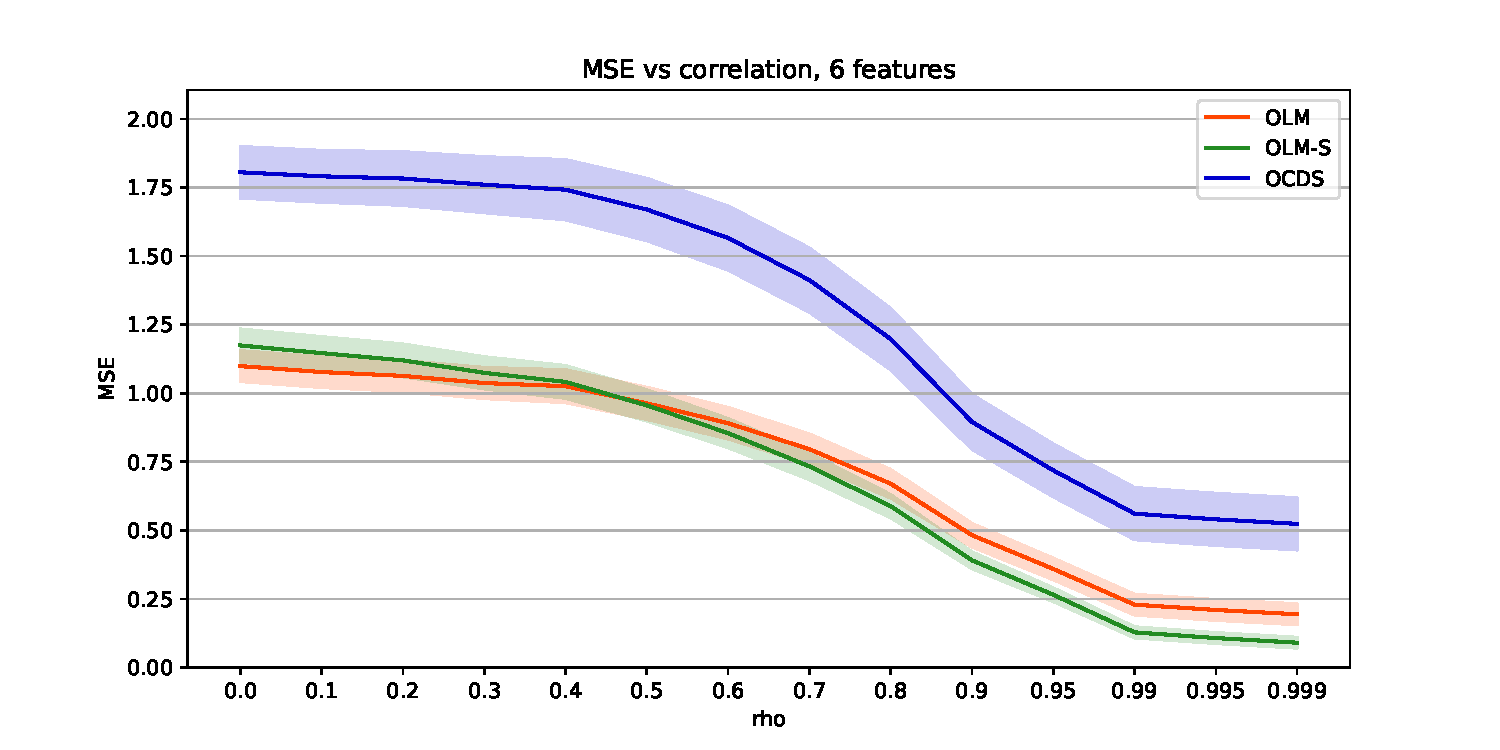
\includegraphics[width=.8\linewidth]{Pictures/sz_200_6_feats_half_missing.pdf}
%     \caption{Average mean square error with confidence intervals for models
%     OLM, OLM-S, and OCDS with varying correlation, tested according to
%     algorithm \ref{alg:test_horizons}, $T=200$, $\Delta T=25$, 6 features + 1
%     constant feature that is always present.}
%     \label{fig:correlation_test_6}
%   \end{subfigure}%
%   \hspace{1em}
% \begin{subfigure}{.4\textwidth}
%   \centering
%   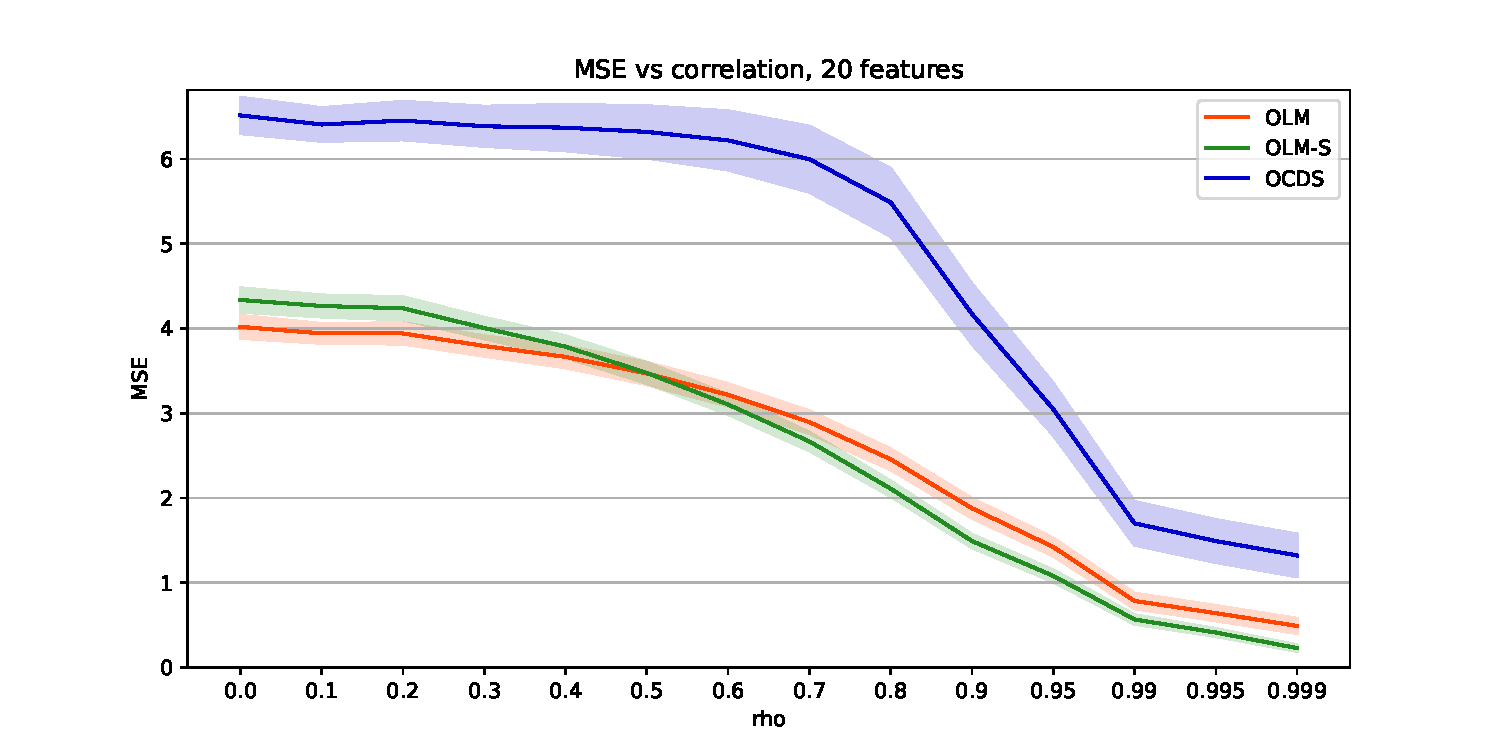
\includegraphics[width=.8\linewidth]{Pictures/sz_200_20_feats_half_missing.pdf}
%     \caption{Average mean square error with confidence intervals for models
%     OLM, OLM-S, and OCDS with varying correlation, tested according to
%     algorithm \ref{alg:test_horizons}, $T=200$, $\Delta T=25$, 20 features + 1
%     constant feature that is always present.}
%   \label{fig:correlation_test_20}
% \end{subfigure}%
%   \caption{Performance of models OLM, OLM-S, and OCDS on synthetic datasets with varying correlation.}
%   \label{fig:correlation_test}
% \end{figure}

\begin{figure}
  \centering
  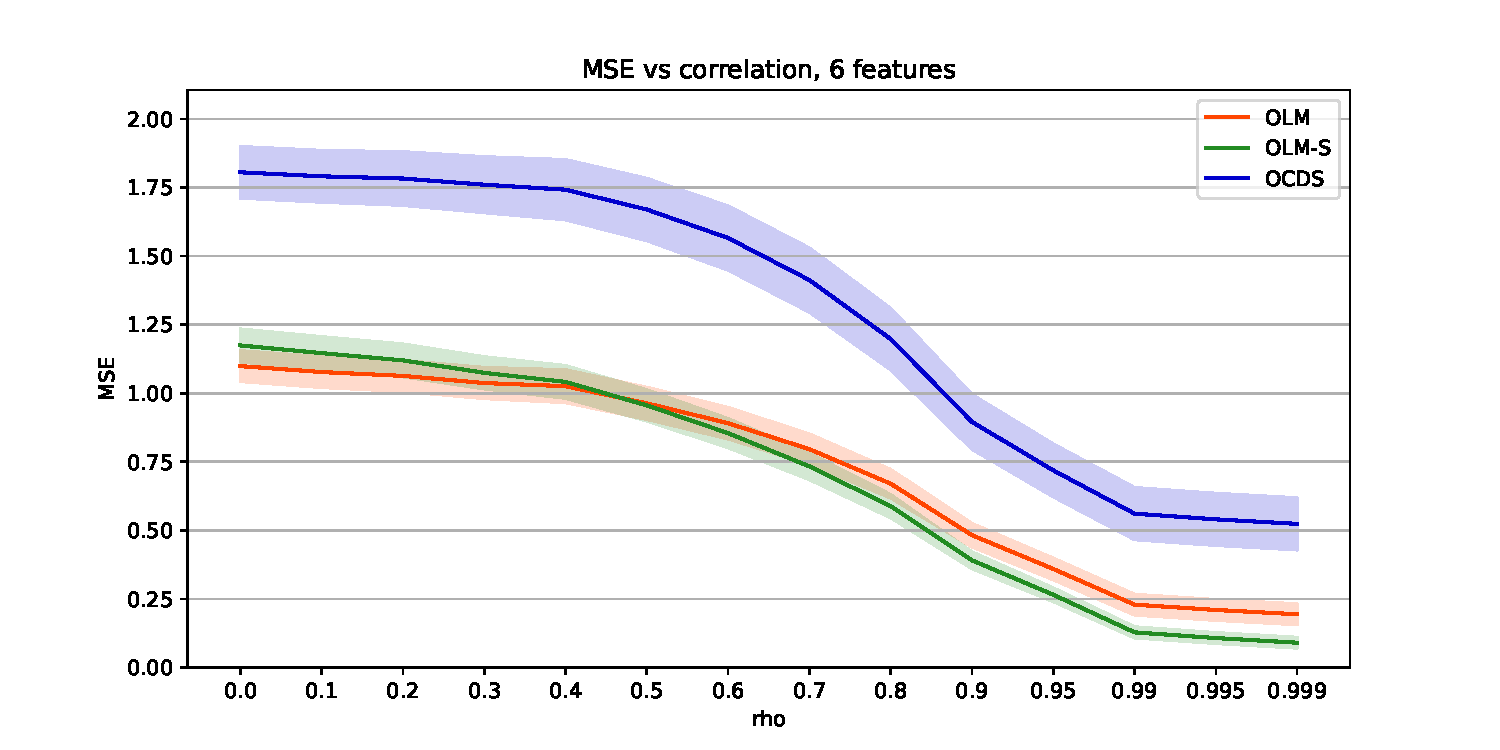
\includegraphics[width=.9\linewidth]{Pictures/sz_200_6_feats_half_missing.pdf}
  \caption{Average mean square error with confidence intervals for models
    OLM, OLM-S, and OCDS with varying correlation, tested according to
    algorithm \ref{alg:test_horizons}, $T=200$, $\Delta T=25$, 6 features.}
  \label{fig:correlation_test_6}
\end{figure}
\begin{figure}
  \centering
  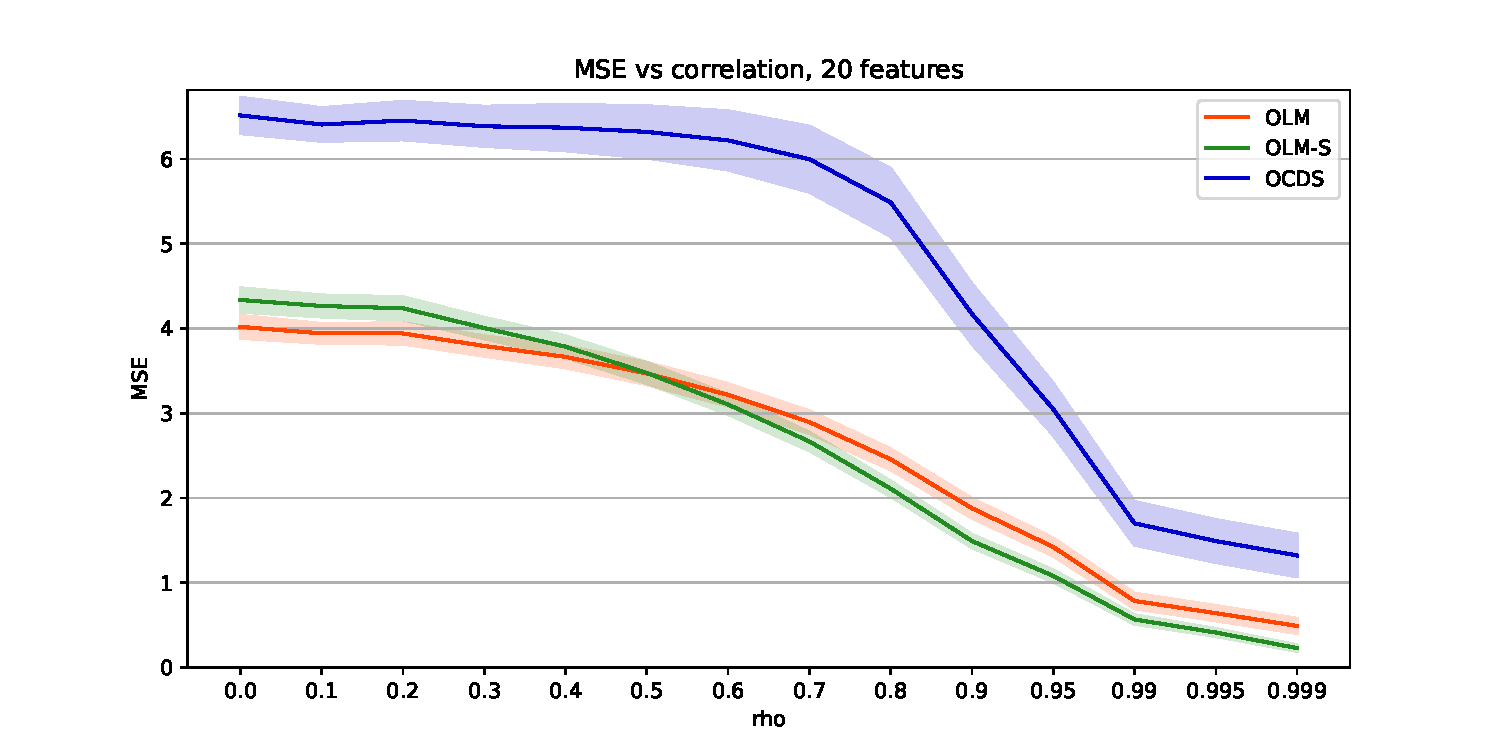
\includegraphics[width=.9\linewidth]{Pictures/sz_200_20_feats_half_missing.pdf}
  \caption{Average mean square error with confidence intervals for models
    OLM, OLM-S, and OCDS with varying correlation, tested according to
    algorithm \ref{alg:test_horizons}, $T=200$, $\Delta T=25$, 20 features.}
  \label{fig:correlation_test_20}
\end{figure}

\subsection{South Carolina Dataset} \label{sec:sc_reg}

Then, I tested the method on a real world dataset. I used the South Carolina
dataset, which is a dataset of 9 geographically colocated wind producers in
South carolina. It contains the hourly production data for the 9 wind farms
over a time span of TODO, given for each wind farm as its percentage production
out of its maximum capacity. The relative locations of the wind farms can be
seen in figure TODO. I no longer test OCDS, since it at no point showed to be
better than OLM or OLM-S.

First, I investigated the dataset, since we want to know whether we expect that
OLM-S can perform well on this dataset. Therefore, I examined the inter-feature
correlation, as seen in figure \ref{fig:sc_corr}. This correlation looks to be in
the high-correlation domain where OLM-S outperformed OLM in the synthetic
dataset. We therefore expect OLM-S to outperform OLM on this dataset as well
when the wind producers from the dataset are used as features.

\begin{figure}
  \centering
  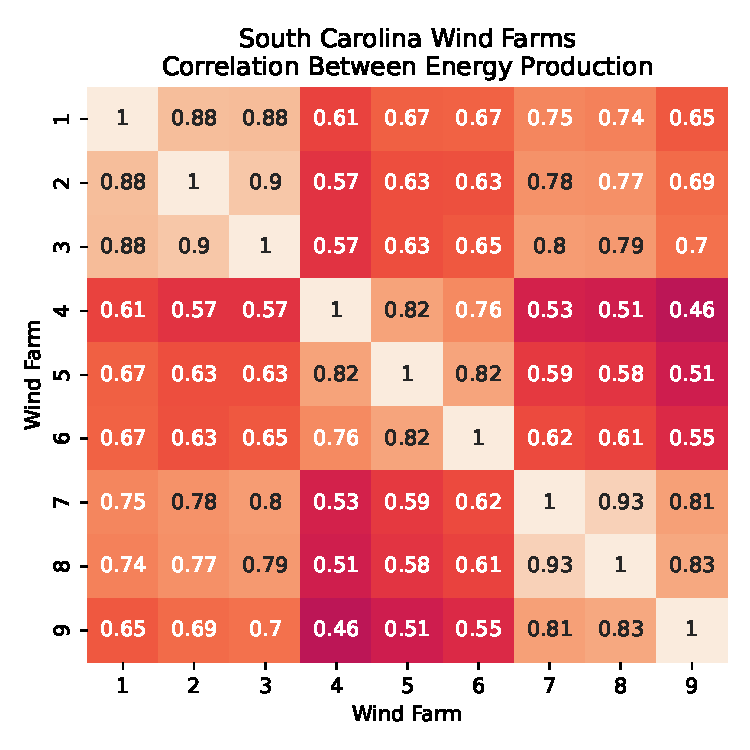
\includegraphics[width=.7\linewidth]{Pictures/south_carolina_corr.pdf}
  \caption{Correlation between $\%$ wind production in the 9 wind farms in the South Carolina dataset.}
  \label{fig:sc_corr}
\end{figure}

I then tested the two models, comparing their average mean square error over
several tests. For every test, I picked 240 observations from the dataset,
equivalent to ten days of observations. I take one of the 9 wind farms and use
its production as the regression target, and then use the production data of
the 8 other wind farms as features with a single hour of lag. I normalize all
features. Similarly to before, I let half of the features be missing from halfway
through the test. For every measurement, I run the test 100 times, each with
a random start time, to generate a more robust prediction as well as
confidence intervals.

The results can be seen in figure \ref{fig:sc}. We see that OLM-S outperforms
OLM for this real world dataset, indicating that there is improvement to be
found by using OLM-S for real world regression markets. We can then create
regression markets with either of the two models OLM and OLM-S, in low and
high-correlation contexts, respectively.

We can then create regression markets with a baseline model for varying feature
spaces in the form of OLM, and a more sophisticated model that reconstructs
missing features in the form of OLM-S when features are more correlated.

\begin{figure}
  \centering
  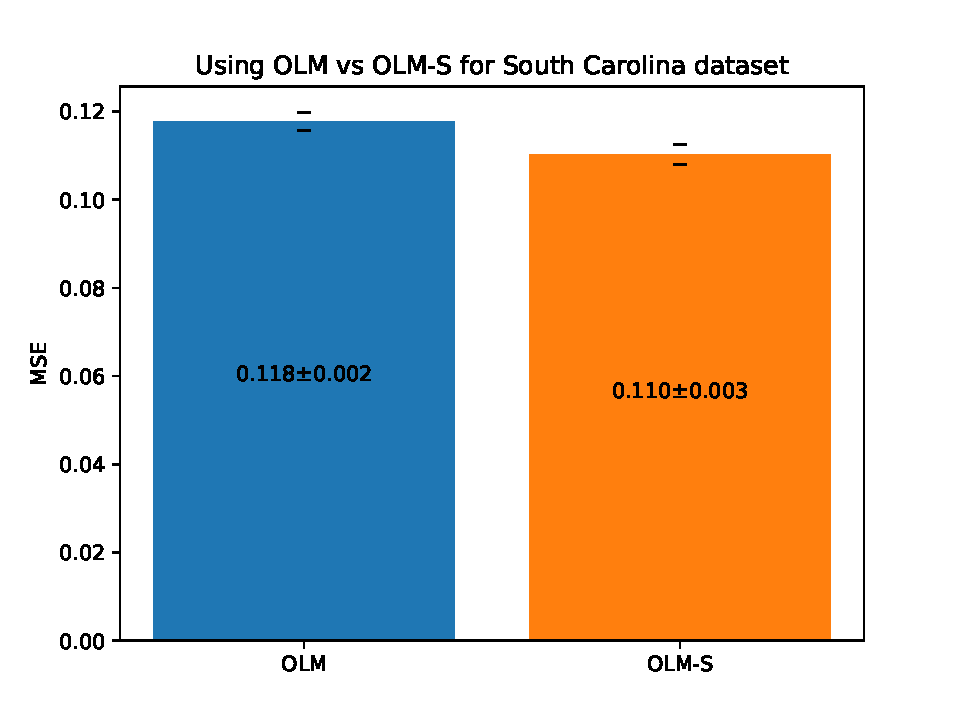
\includegraphics[width=.7\linewidth]{Pictures/south_carolina.pdf}
  \caption{Average MSE over 100 tests on the South Carolina dataset, using OLM
    and OLM-S. 1 step ahead forecasting. The loss using OLM-S is significantly
    lower than the loss using OLM.}
  \label{fig:sc}
\end{figure}

TODO: EXPLAIN WHERE SOUTH CAROLINA DATASET COMES FROM.

TODO: INTRODUCE TIME-AHEAD FOR RECONSTRUCTION MODELS EARLIER

\section{Regression Market}
In this section, I present results for running a regression market as described
in section TODO:CREATE SECTION IN PRELIMINARIES, using the OLM and OLM-S models
for its function. I compare using reconstruction as seen in OLM-S with the
baseline OLM. I also investigate the structure of the distributed revenue
including instances of negative payment, how revenue is increased from feature
reconstruction, and the effects of mean imputation on revenue distribution.

The always-present constant feature is given to the central agent as its only feature.

\subsection{Synthetic Dataset}

In this section, I show the results of using either the OLM or the OLM-S
methods as market models in situations with missing data. I use a setup as seen
in the regression section, algorithm \ref{alg:test_horizons}. I set the buyer's
willingness to pay to 1. I generate the dataset and run the market TODO times,
to generate confidence intervals for the observations.

An example run of the market is shown in figure \ref{fig:market_example}. We
see the cumulative payouts for each feature, as well as how the coefficients of
the model change over time. The missing features are reconstructed each time step.

\begin{figure}
  \centering
  \begin{subfigure}{.4\textwidth}
    \centering
    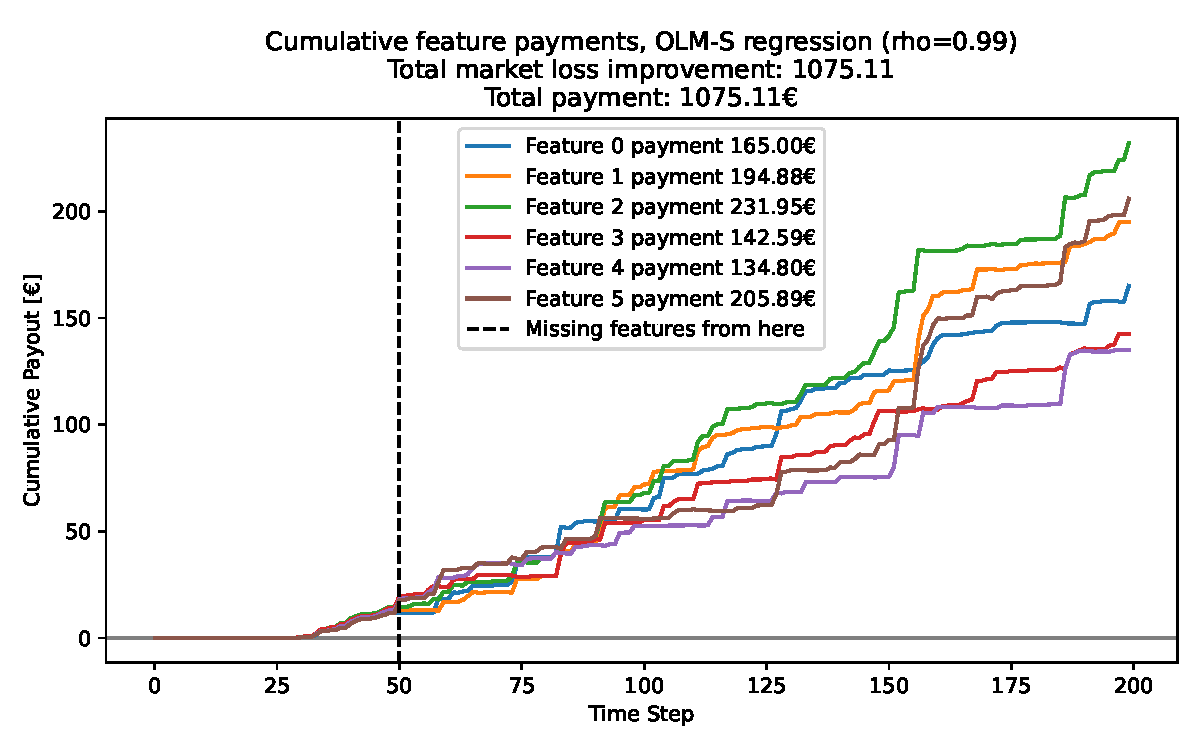
\includegraphics[width=.9\linewidth]{Pictures/cumulative_payments.pdf}
    \caption{TODO}
    \label{fig:cumulative_payments}
  \end{subfigure}%
  \hspace{1em}
  \begin{subfigure}{.4\textwidth}
    \centering
    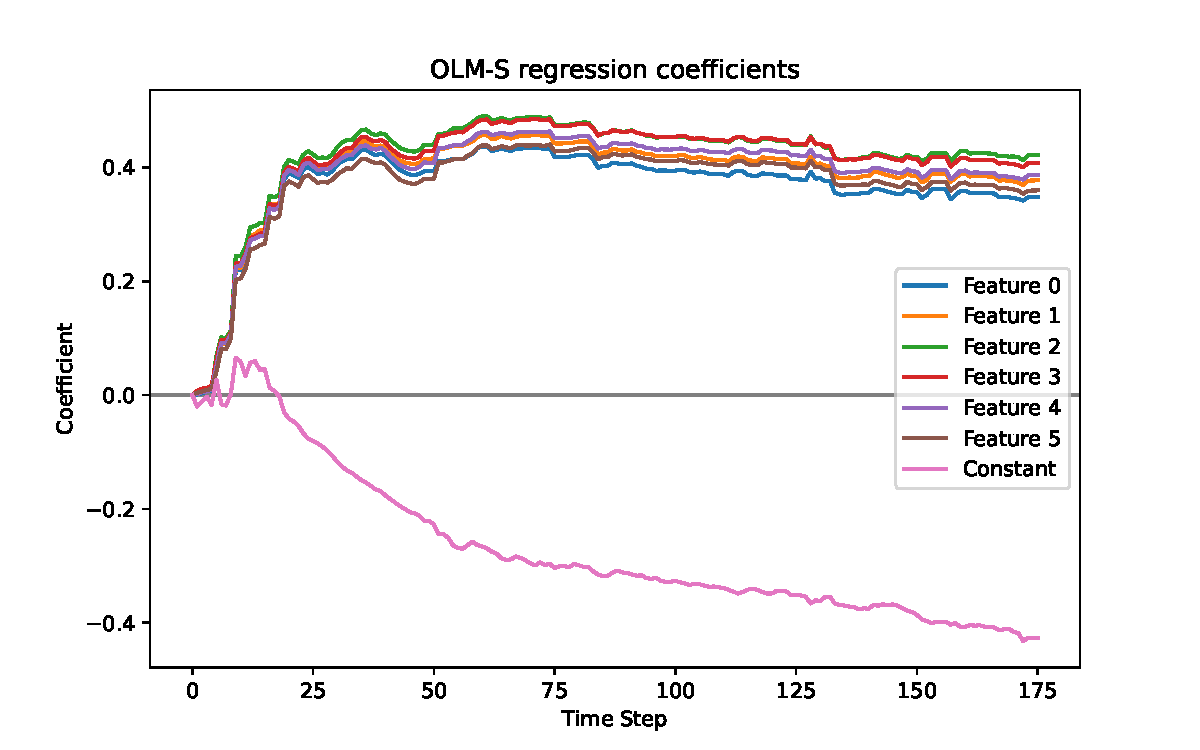
\includegraphics[width=.9\linewidth]{Pictures/regression_coefficients.pdf}
    \caption{TODO}
    \label{fig:regression_coefficients}
  \end{subfigure}%
  \caption{An example run of a regression market on a synthetic dataset
    generated as described earlier, following the method in algorithm
    \ref{alg:test_horizons}, $T=200$, $\Delta T=25$, using the OLM-S regressor.
    Shows both cumulative payments over time, as well as the regression
    coefficients for the six features present.}
  \label{fig:market_example}
\end{figure}

To investigate the out-of-sample outcome of using OLM-S versus OLM in the
market, I ran the market several times, and the average feature payments using
market models OLM and OLM-S in a high correlation context are shown in figure
\ref{fig:payout_high_corr}. All features are paid better using reconstruction
than leaving out reconstruction. Note that if all market participants mean
impute, the OLM-S method reduces to OLM. We can see how market participants are
incentivized, then, to truthfully report their features as missing. However,
when correlations are low, we know that OLM outperforms OLM-S, so participants
are actually incentivized to mean impute when their feature does not correlate
much with other features.

% low, $\rho=TODO$. Here, we see that features are paid better using OLM than
% OLM-S. The OLM-S market is thus only superior in situations where features are
% highly correlated.

\begin{figure}
  \centering
  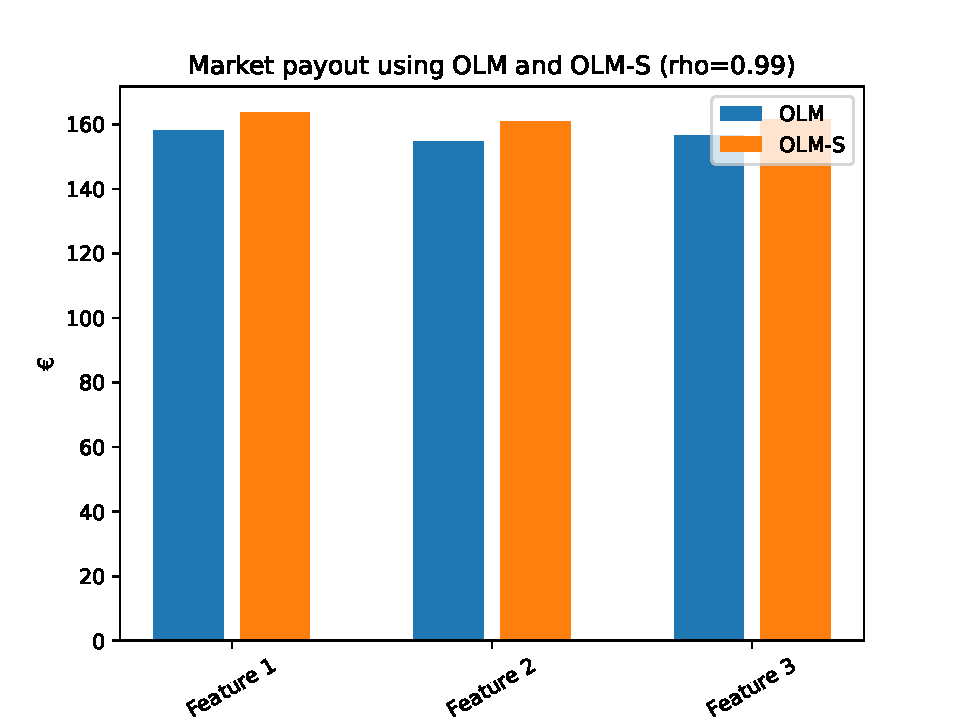
\includegraphics[width=.9\linewidth]{Pictures/payout_rho099.pdf}
  \caption{Average payment for each feature over 100 runs of the market, generating predictions using algorithm \ref{alg:test_horizons}, $T=200$, $\Delta T=25$, 3 features. The difference in the mean payments for the features are statistically all significant in a paired t-test with $p<1^{-10}$.}
  \label{fig:payout_high_corr}
\end{figure}



Feature owners sometimes receive negative Shapley values. The fraction of
negative payments and the sum negative payments distributed by OLM and OLM-S
are shown in figure \ref{fig:negative_payments}. We see that the risk of having
to pay back to the market is much smaller when using OLM-S as the regression
mechanism. For a risk-averse agent, this is a bonus of using OLM-S as the
market mechanism, and brings us closer to an ex-post individually rational
market.

\begin{figure}
  \centering
  \begin{subfigure}{.4\textwidth}
    \centering
    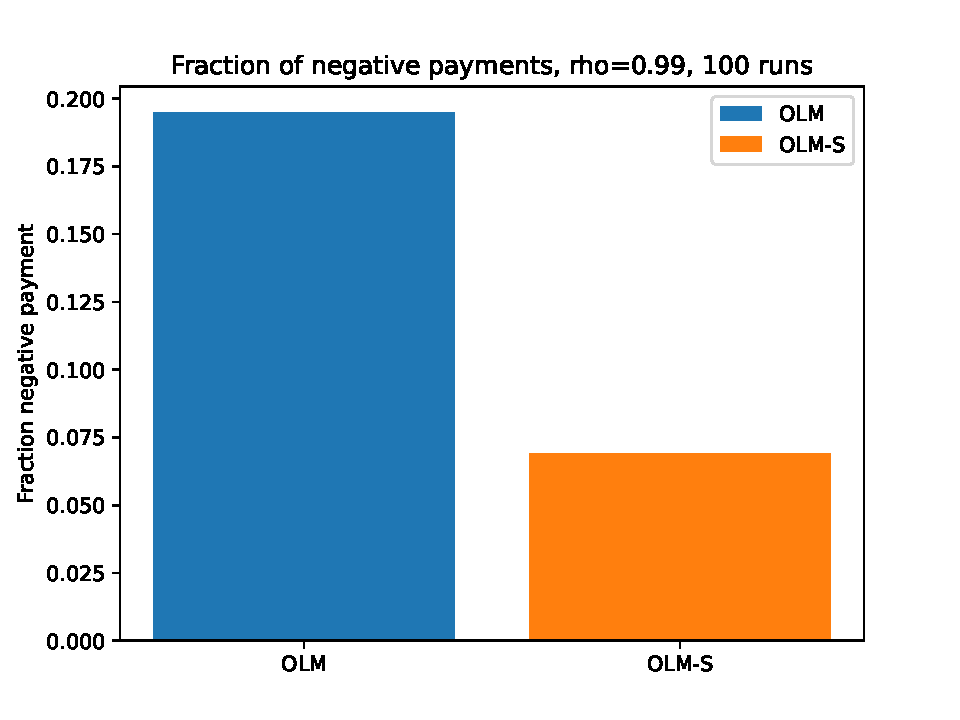
\includegraphics[width=.9\linewidth]{Pictures/negative_fraction.pdf}
    \caption{Fraction of all payments to feature sellers that are negative.}
    \label{fig:negative_fraction}
  \end{subfigure}%
  \hspace{1em}
  \begin{subfigure}{.4\textwidth}
    \centering
    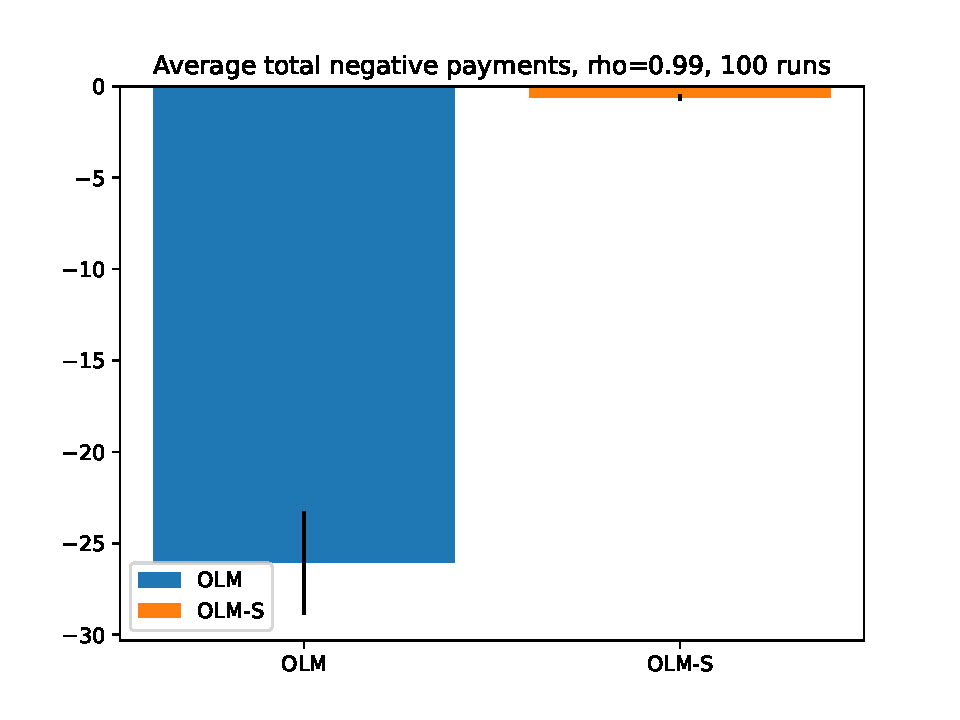
\includegraphics[width=.9\linewidth]{Pictures/negative_total.pdf}
    \caption{Total negative payments given out in a single run of the market.}
    \label{fig:negative_total}
  \end{subfigure}%
  \caption{Fraction of negative payments and total negative payments per run, over
    100 runs of the market, generating a synthetic dataset and using algorithm
    \ref{alg:test_horizons}, $T=200$, $\Delta T=25$, 3 features.}
  \label{fig:negative_payments}
\end{figure}

% We expect for sellers to
% receive negative payoffs when their features are missing, so I investigated
% seller payment when their feature is missing. This is shown in figure
% TODO:FIGURE. From these figures, we see that feature owners mostly receive
% negative payment when they do not supply their feature to the market TODO. This
% matches our expectation TODO: SHOW THAT THIS MATCHES EXPECTATION IN PRELIM/CONTRIB.

\subsection{Payment for missing features}

Features still get shapley values assigned to them when they are missing. We
can show that the Shapley values for missing features are expected to be zero
in-sample todo. I have illustrated the payment received by missing features in figure \ref{fig:missing_features}. From this, we see that using OLM-S makes the payments to missing features less negative, and actually makes them positive. This is favorable for participants, since it again means less risk for market participants. TODO: SHOULD I TALK ABOUT IT GETTING CLOSER TO 0 WITH MORE FEATURES

% In figures TODO and TODO, I have illustrated the payments over
% the course of a test for OLM and OLM-S features when correlations are low and
% high, respectively. As expected, low correlation leads to near-zero shapley
% values when features are missing. High correlation leads to small positive
% payments for OLM-S when there are few features, and near-zero payments for more
% features. From the theory TODO, we expect zero Shapley values for few features.

\begin{figure}
  \centering
  \begin{subfigure}{.4\textwidth}
    \centering
    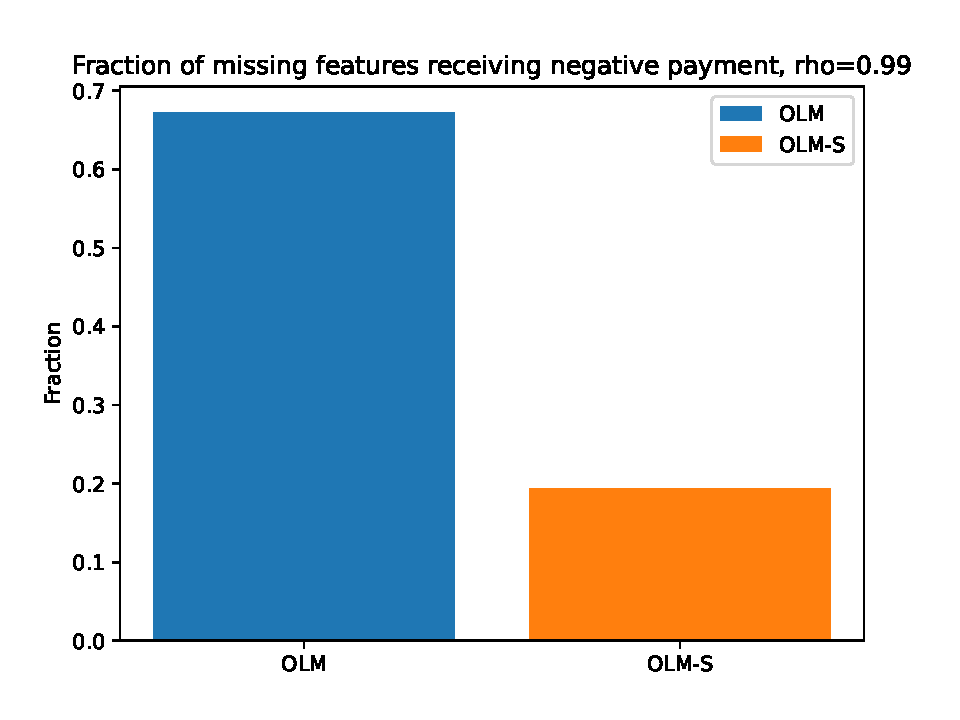
\includegraphics[width=.9\linewidth]{Pictures/missing_negative_fraction.pdf}
    \caption{Fraction of single time-step payments to missing features that are negative.}
    \label{fig:missing_negative_fraction}
  \end{subfigure}%
  \hspace{1em}
  \begin{subfigure}{.4\textwidth}
    \centering
    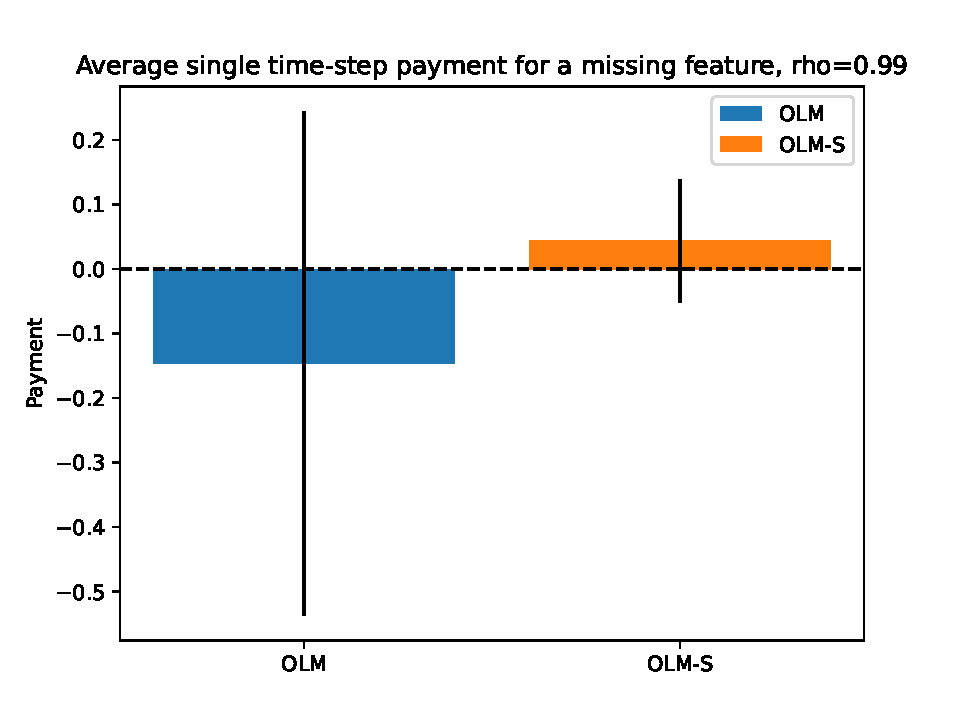
\includegraphics[width=.9\linewidth]{Pictures/missing_payment.pdf}
    \caption{The average single time-step payment to missing features across
      all time steps and runs. Error bars indicate the standard deviation.}
    \label{fig:missing_payment}
  \end{subfigure}%
  \caption{Payments for missing features for a hundred runs of the market using a synthetic dataset. Following algorithm \ref{alg:test_horizons}, $T=200$, $\Delta T=25$, 3 features. For comparison, every time step that a feature is present in the above, it is paid on average $1.12$ by OLM and $1.08$ by OLM-S, meaning that payments for missing features are of a much smaller magnitude.}
  \label{fig:missing_features}
\end{figure}
% I suspect that the positive Shapley values when there are very few features
% comes from a kind of regularizing effect of the missing features. I cannot
% prove or theoretically found this, though. The payments are very small, the
% total payment is on average TODO, while the average sum payment for missing
% features is on average TODO.

\subsection{Gains from Reconstruction}

Feature revenue is increased in OLM-S by reconstruction of other features.
Using a Shapley value approach we can decompose the gained revenue for each
feature by reconstructing each other feature. This approach is described in
algorithm \ref{alg:revenue_decomposition}.


\begin{algorithm}
  \caption{Pseudocode for decomposing revenue gain by feature.}\label{alg:revenue_decomposition}
  \begin{algorithmic}
    \State Generate $X,y$ synthetically based on number of features and $\rho$

    \For{$\omega \in S$} %TODO: ENSURE THAT THIS IS CORRECT
    \State Initialize OLM-S model $m_{\omega}$ that only reconstructs
    features $\omega$
    \State Calculate payment $\pi_{i,\omega}$ for each feature $i$ using
    model $m_{\omega}$ and dataset $X,y$
    \EndFor

    \For{$i \in U$} %TODO: NOTATION FOR ALL FEATURES
    \State Calculate Shapley value $\psi_{i,j}$ for each feature $j$ where
    the payoff for each coalition $\omega$ is $\pi_{i,\omega}$
    \EndFor
    \State Shapley values $\psi_{i,j}$ show contribution to payment to feature
    $i$ from the algorithm reconstructing feature $j$
  \end{algorithmic}
\end{algorithm}

The revenue breakdown from reconstructing each feature is shown in figure TODO:
REF FIG. We see that a feature has its revenue considerably increased by being
reconstructed, but decreased by reconstructing other features. Since we know
that payments are very small at time steps where features are missing, This
indicates that reconstruction keeps feature coefficients of high quality while
a feature is missing, so that it can continue performing when it reenters the
market. Reconstruction is thus a service that the rest of the features perform
for the missing feature. This might make one think again of the revenue
distribution idea presented in section TODO:REF, where the Shapley value of a
missing feature is distributed between the present features. This result
however further shows why this revenue distribution method cannot be used:
Features will have near-zero or negative Shapley values when they are missing,
but will then have a higher Shapley value than without reconstruction once they
return, so reconstructing features would in this case get their revenue
decreased in exchange for increasing the revenue of the missing features once
they return to the market.

\begin{figure}
  \centering
  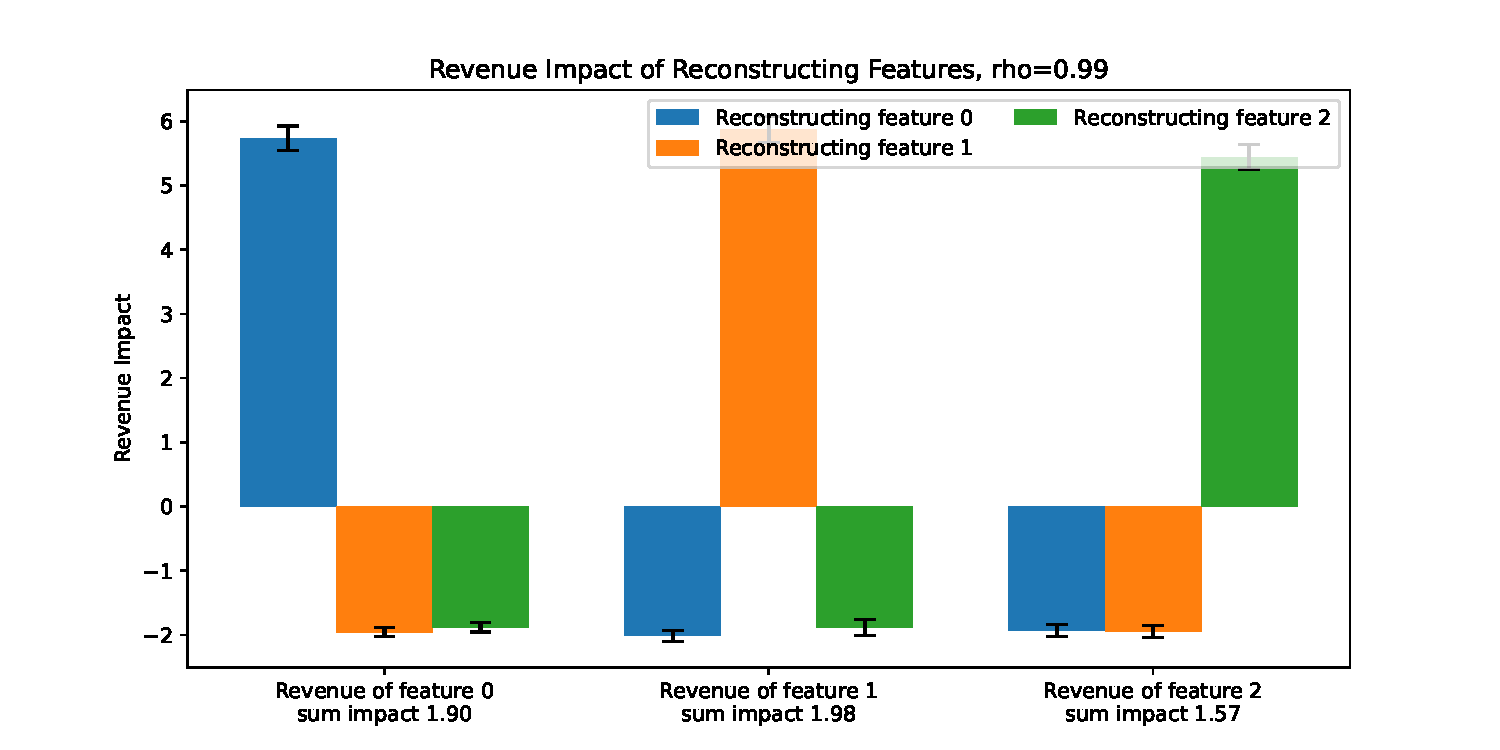
\includegraphics[width=.9\linewidth]{Pictures/reconstruction_impact.pdf}
  \caption{Impact to feature revenue from reconstructing other features,
    calculated by algorithm \ref{alg:revenue_decomposition}. From fifty runs of
    the market, using algorithm \ref{alg:test_horizons}, $T=200$, $\Delta T=25$,
    3 features.}
  \label{fig:revenue_impact}
\end{figure}




\subsection{Truthfulness under Imputation}
TODO : THIS SECTION IS UP FOR DELETION / CHANGE

When a feature is missing, participants in the market have the option to mean
impute their missing information based on historical data. This is as mentioned
uninformative, and we have already shown that it does not hold in-sample
in-expectation. In figure TODO, the results of mean imputation are shown in a
high correlation setting. We see that mean imputation causes OLM-S to reduce to
the OLM algorithm, and they perform the same. This interestingly means that
even though we have truthfulness under imputation in-sample in-expectation, we
actually expect empirically for truthfulness under imputation to disappear in
low-correlation out-of-sample contexts, based on our regression results in
section TODO. This is because in these contexts, OLM ourperforms OLM-S, and
mean imputation reverts OLM-S to OLM, so it is incentivized.

TODO: DESCRIBE CONSEQUENCES OF LOSING TRUTHFULNESS UNDER IMPUTATION

TODO: ALSO SHOW RESULT OF NOT PAYING MISSING FEATURES

TODO: IS TRUTHFULNESS UNDER IMPUTATION REALLY THAT INTERESTING?

\subsection{South Carolina Dataset}
In this section, I show example market results when the dataset is the South
Carolina wind farm dataset as described in section \ref{sec:sc_reg}.
The results are shown in figure \ref{fig:south_carolina_market}.

\begin{figure}
  \centering
  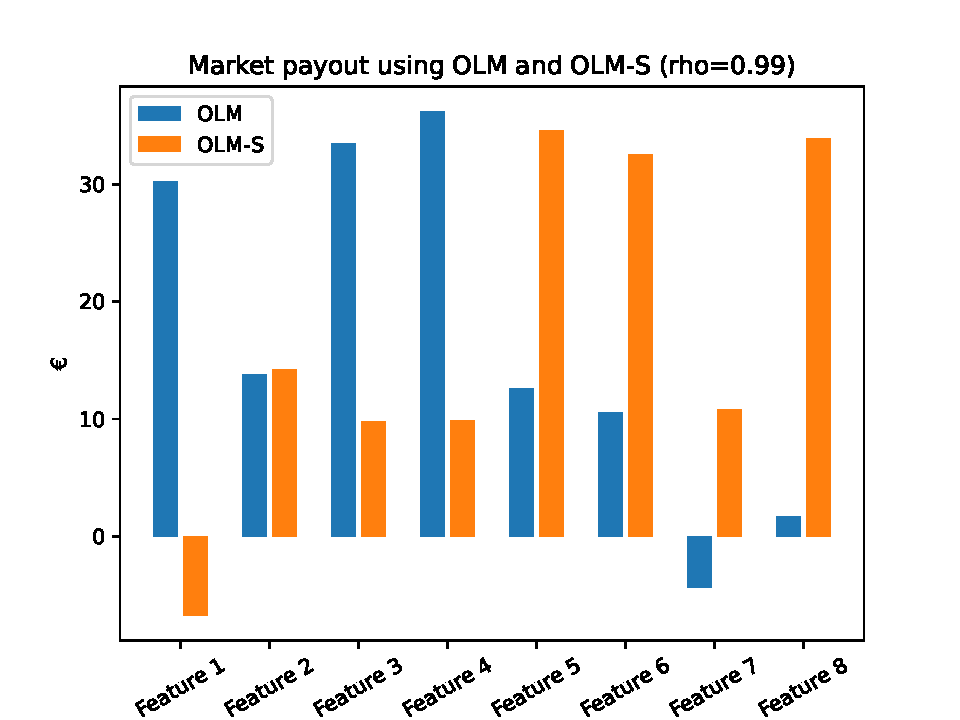
\includegraphics[width=.9\linewidth]{Pictures/south_carolina_market.pdf}
  \caption{TODO WHY DO ALL THE FEATURES LOSE MONEY, AND WHY ARE SO MANY FEATURES GETTING NEGATIVE PAYMENTS???}
  \label{fig:south_carolina_market}
\end{figure}

TODO: I NEED TO CHANGE SETUP, IT SHOULD ALSO HAVE ITS OWN PRODUCTION DATA AVAILABLE AS CENTRAL AGENT FEATURE
TODO
